\section{Introduction}

\begin{frame}{Motivation}
\begin{itemize}
    \item Graph machine learning can be tracked backwards to the problem of `learning' on data that is inherently a graph \cite{silva2016machine, JMLR:Perozzi} or can be modeled as a graph \cite{verri2013,grape2020}
    \item Variety of tasks:  node/edge classification, link prediction, graph partitioning, which rely on learning representations from graph-structured data.
    \item  Techniques were most developed by complex networks researchers.
    \item \textbf{Last decade:} significant shift towards the merging of three main communities: graph signal processing, deep learning and complex nets.
    
\end{itemize}
\end{frame}

\begin{frame}{GraphML paradigms Overview}
    \begin{itemize}
        \item Three main learning paradigms: supervised, unsupervised, and semi-supervised learning
        \item We are interested on the (semi-)supervised learning paradigm, which encompasses a variety of techniques designed to leverage learning to (partially-)labeled data \cite{verri2018advantages,amanciof}
        \item  Focus in the subset of graph elements (nodes,edges,graph structure) prediction(classification/regression) methods.
        \item Consider the division of the field into \texttt{traditional} graph learning and \texttt{deep} graph learning
        
    \end{itemize}
    \end{frame}

\begin{frame}{Introduction to Last-Mile Delivery Drones}
    \begin{figure}
      \begin{columns}
        \column{.3\linewidth}
        \caption{Drones Congestion in a high-traffic Last Mile Delivery context. \\ Source: \cite{imageDronesCongestion}}
        \label{fig:example left}
        \column{.65\linewidth}
        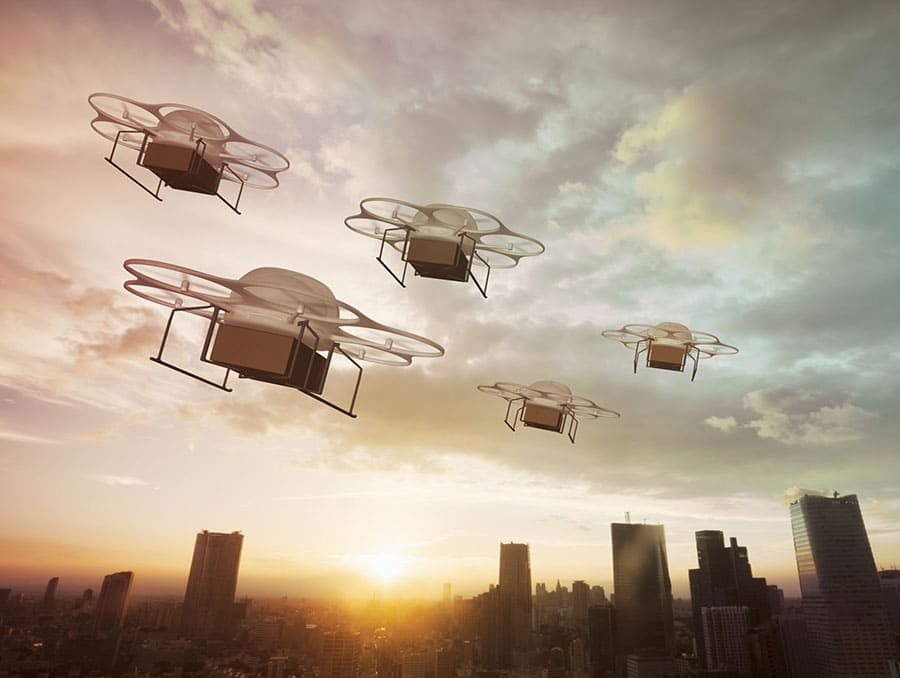
\includegraphics[width=\textwidth]{img/Drone Congestion.jpg}
      \end{columns}
    \end{figure}

\end{frame}

\begin{frame}{Introduction to Last-Mile Delivery Drones}
\destaq{Last Mile Delivery Drones (LMDD)}
\begin{itemize}
    \item Heterogeneous research area:
    \begin{itemize}
        \item Combining drones and trucks.
        \item Linear integer modeling.
        \item Fuzzy logic for uncertainties.
        \item Multi-objective optimization.
        \item Exclusive drone-based solutions.
    \end{itemize}
    \item \textbf{Complex Systems Decentralized Approach}:
    \begin{itemize}
        \item Tradable permit model for multi-agent airspace use \cite{Verri}.
    \end{itemize}
\end{itemize}

\end{frame}

\begin{frame}{Related Work and Centralized Control}
\begin{itemize}
    \item \textbf{Necessity of Air Traffic Management}:
    \begin{itemize}
        \item Most centralized models don't address collision avoidance \cite{DUKKANCI2023}.
        \item Ensuring optimal path planning and efficient airspace control.
    \end{itemize}
    \item \textbf{Centralized Control and UTM}:
    \begin{itemize}
        \item \textbf{Centralized Control}:
        \begin{itemize}
            \item Federal Aviation Administration (FAA) and NASA's Unmanned Aircraft System Traffic Management (UTM) \cite{nasa}.
            \item Ensures organized, legislative-backed airspace control.
        \end{itemize}
        \item \textbf{Decentralized Models}:
        \begin{itemize}
            \item Novel but complex in scalability and regulatory compliance.
        \end{itemize}
    \end{itemize}
\end{itemize}
\end{frame}


\begin{frame}{Proposed Approach}
\begin{itemize}
    \item \textbf{Aispace Control and MAPF Approach}:
    \begin{itemize}
        \item Multi-Agent Path Finding (MAPF) is a solution for addressing spatial characteristics and collision avoidance.
    \end{itemize}
    \item \textbf{Proposed Strategy}:
    \begin{itemize}
        \item Employing MAPF strategy for Last Mile Delivery Drone problem.
        \item Three approaches: MILP, heuristic and hybrid.
        \item Use of prioritized planning \cite{7138650} and conflict-based search \cite{SHARON201540} to manage computational complexity in the heuristic.
        \item Comparing the MILP with the heuristic.
        \item Qualitative comparison between centralized and decentralized approaches.
    \end{itemize}
\end{itemize}
\end{frame}


